\documentclass[../DoAn.tex]{subfiles}
\begin{document}

\section{Thiết kế kiến trúc}
\subsection{Lựa chọn kiến trúc phần mềm}
Sau khi nghiên cứu, xem xét kĩ các yêu cầu của hệ thống, ĐATN chọn mô hình MVC làm kiến trúc cho hệ thống của mình. Hình 4.1 đưới đây minh họa luồng hoạt động tổng quan của mô hình MVC:
\begin{figure}[H]
    \centering
    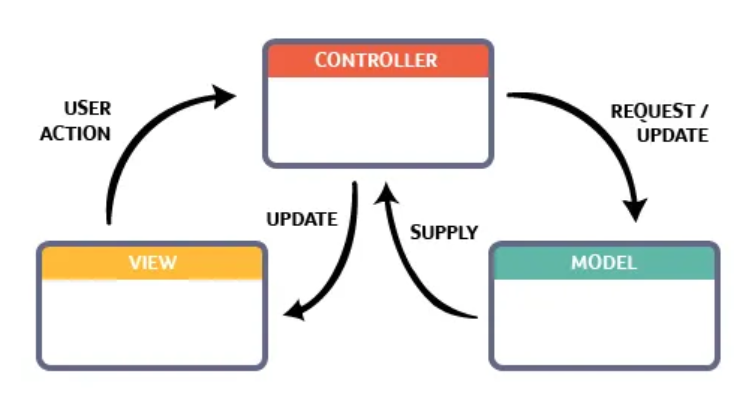
\includegraphics[width=0.65\linewidth]{Hinhve/MVC.png}
    \caption{Luồng hoạt động của mô hình MVC}
    \label{fig:Fig1}
\end{figure}

MVC (Model-View-Controller) là mẫu kiến trúc phần mềm trên máy tính nhằm mục đích tạo lập giao diện cho người dùng \cite{deacon2009model}. Theo đó, hệ thống MVC được chia thành ba phần có khả năng tương tác với nhau và tách biệt các nguyên tắc nghiệp vụ với giao diện người dùng. Ba thành phần ấy bao gồm:
\begin{itemize}
    \item Controller giữ nhiệm vụ nhận điều hướng các yêu cầu người dùng và gọi những phương thức xử lý chúng. 
    \item Model hay còn được gọi tầng dữ liệu là thành phần chứa tất cả các nghiệp vụ logic, phương thức xử lý, truy xuất database, đối tượng mô tả dữ liệu như các Class, hàm xử lý,...
    \item View đảm nhận việc hiển thị thông tin, nhận yêu cầu từ người dùng, nơi chứa tất cả đối tượng GUI như textbox, image,...
\end{itemize}
Bằng cách này, thông tin nội hàm được xử lý tách biệt với phần thông tin xuất hiện trong giao diện người dùng. Ngoài ra, mô hình này còn có các ưu điểm: 
\begin{itemize}
    \item Dễ dàng rà soát lỗi: Do luồng hoạt động rõ ràng, các lỗi phát sinh dễ dàng được tìm thấy, đảm bảo chất lượng cho phần mềm.
    \item Đơn giản: Mô hình phân chia công việc với các chức năng rõ ràng, kết cấu đơn giản cho người lập trình.
\end{itemize}
\newpage
\subsection{Thiết kế tổng quan}
\begin{figure}[H]
    \centering
    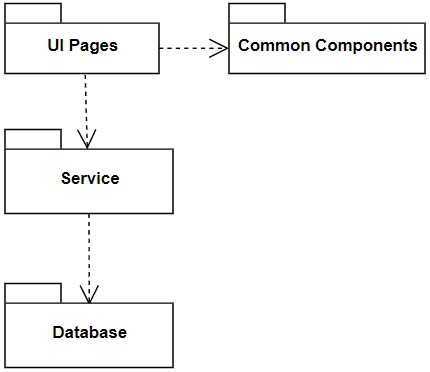
\includegraphics{Hinhve/package.png}
    \caption{Biểu đồ phụ thuộc gói}
    \label{fig:Fig1}
\end{figure}
Thiết kế tổng quan của hệ thống bao gồm bốn gói bao gồm: UI Pages, Common Components, Service và Database. Gói Common Components chứa các thành phần giao diện chung được sử dụng trong gói UI Pages. UI Pages chứa các thành phần giao diện diện chính của hệ thống mà sẽ được hiển thị trực tiếp phía người dùng. Gói Service chứa các thành phần chịu trách nhiệm nhận, điều hướng và xử lý các nghiệp vụ nhận được từ phía người dùng thông qua các thành phần giao diện. Gói Database chứa các thành phần tương tác với cơ sở dữ liệu.
\newpage
\subsection{Thiết kế chi tiết gói}
\begin{figure}[H]
    \centering
    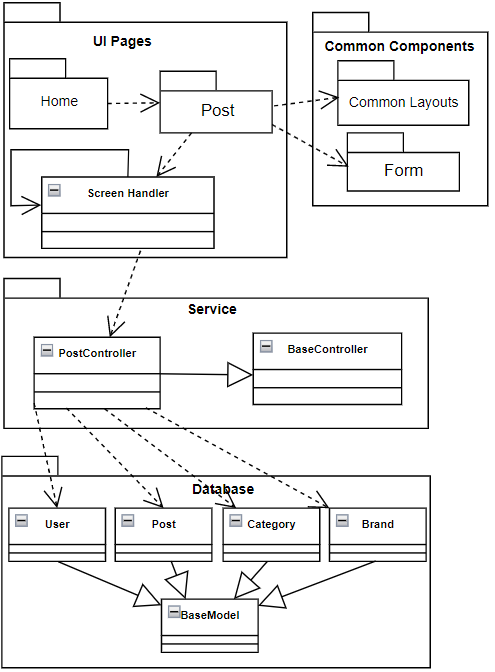
\includegraphics[width=0.9\linewidth]{Hinhve/package-detail.png}
    \caption{Sơ đồ thiết kế gói ứng với chức năng đăng bài viết}
    \label{fig:Fig1}
\end{figure}
Đối với các chức năng trong hệ thống, cả bốn gói đều có thành phần tham gia chịu trách nhiệm của từng tầng trong mô hình MVC. Cụ thể với ví dụ về chức năng đăng bài viết, ứng với tầng Giao diện (View) có 2 gói tham gia là UI Pages và Common Components. Trong đó, tầng UI Pages có 2 thành phần giao diện tham gia đó là Home và Post, đồng thời chúng sử dụng các thành phần dùng chung là Common Layouts và Form trong gói Common Componets. Ngoài ra, trong gói này có lớp Screen Handler chịu trách nhiệm chuyển tiếp giữa các giao diện tĩnh đồng thời gửi yêu cầu đến tầng Nghiệp vụ (Controller). Tầng Nghiệp vụ có gói tương ứng là Service. Trong chức năng này, lớp PostController kế thừa lớp BaseController và thực hiện các chức năng nhận thông tin, xử lý logic và yêu cầu dữ liệu từ tầng dữ liệu. Gói Database trong thiết kế tổng quan chính là tầng Dữ liệu trong kiến trúc MVC. Ở chức năng này, các model tham gia quá trình xử lý bao gồm User, Post, Category và Brand.
\section{Thiết kế chi tiết}
\subsection{Thiết kế giao diện}
Mục này trình bày về các thông số quan trọng của màn hình trong hệ thống. Mục đích của việc này là để đảm bảo tính nhất quán trong từng chi tiết khi thiết kế giao diện cho hệ thống. Kết quả cuối cùng là một trang web được tối ưu cho trải nghiệm người dùng một cách tốt nhất. Đồng thời, mục này sẽ trình bày một số thiết kế một số giao diện chính bằng công cụ Mockup.

\subsubsection{Các thông số quan trọng của màn hình}
\begin{table}[H]
\begin{tabular}{|p{1cm}|p{4cm}|p{9cm}|}
\hline
STT & Thông tin           & Các thông số màn hình                                                                                                                                                                                                                                            \\ \hline
1   & Kích thước màn hình & \begin{tabular}[c]{@{}l@{}}Máy tính bàn: \\ (Desktops - Medium devices): \textgreater{}= 992px\\ Máy tính lớn: \\ (Large Desktops - Large devices) \textgreater{}= 1200px\end{tabular}                                                                           \\ \hline
2   & Màu sắc màn hình    & \begin{tabular}[c]{@{}l@{}}Màu nền: \#f7fafc\\ Màu tiêu đề: \#1a202c\\ Màu chữ thường: \#1a202c\\ Màu nút chính: \#2c5282\\ Màu nút chính khi di chuyển chuột vào: \#2b6cb0\\ Màu nút phụ: \#edf2f7\\ Màu nút phụ khi di chuyển chuột vào: \#e2e8f0\end{tabular} \\ \hline
3   & Kiểu chữ            & SF Pro Display                                                                                                                                                                                                                                                   \\ \hline
4   & Ngôn ngữ            & Tiếng Việt                                                                                                                                                                                                                                                       \\ \hline
\end{tabular}
\caption{Thông số của màn hình khi thiết kế giao diện người dùng}
\label{tab:my-table}
\end{table}
\newpage
\subsubsection{Một số thiết kế các màn hình quan trọng}
\begin{figure}[H]
    \centering
    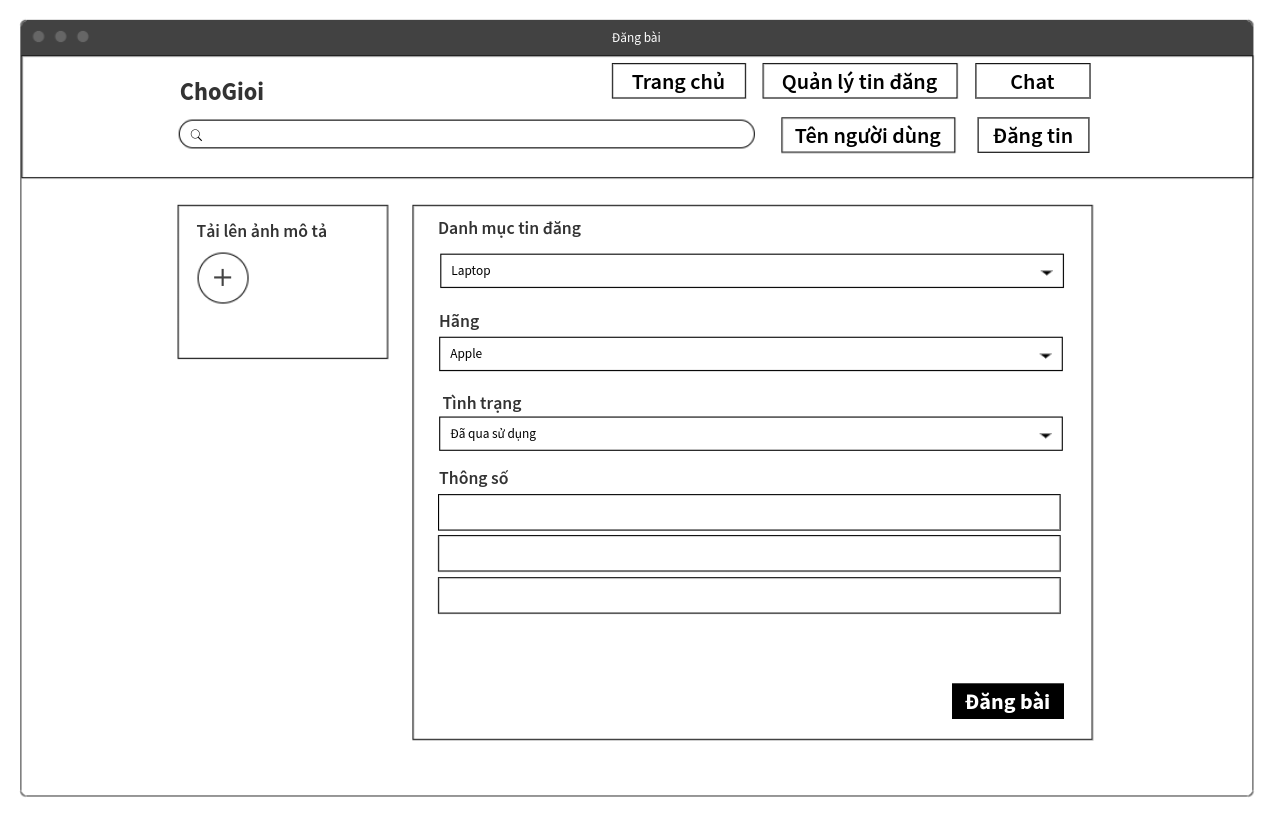
\includegraphics[width=0.8\linewidth]{Hinhve/AddPost.png}
    \caption{Wireframe màn hình Đăng bài}
    \label{fig:Fig1}
\end{figure}
\begin{figure}[H]
    \centering
    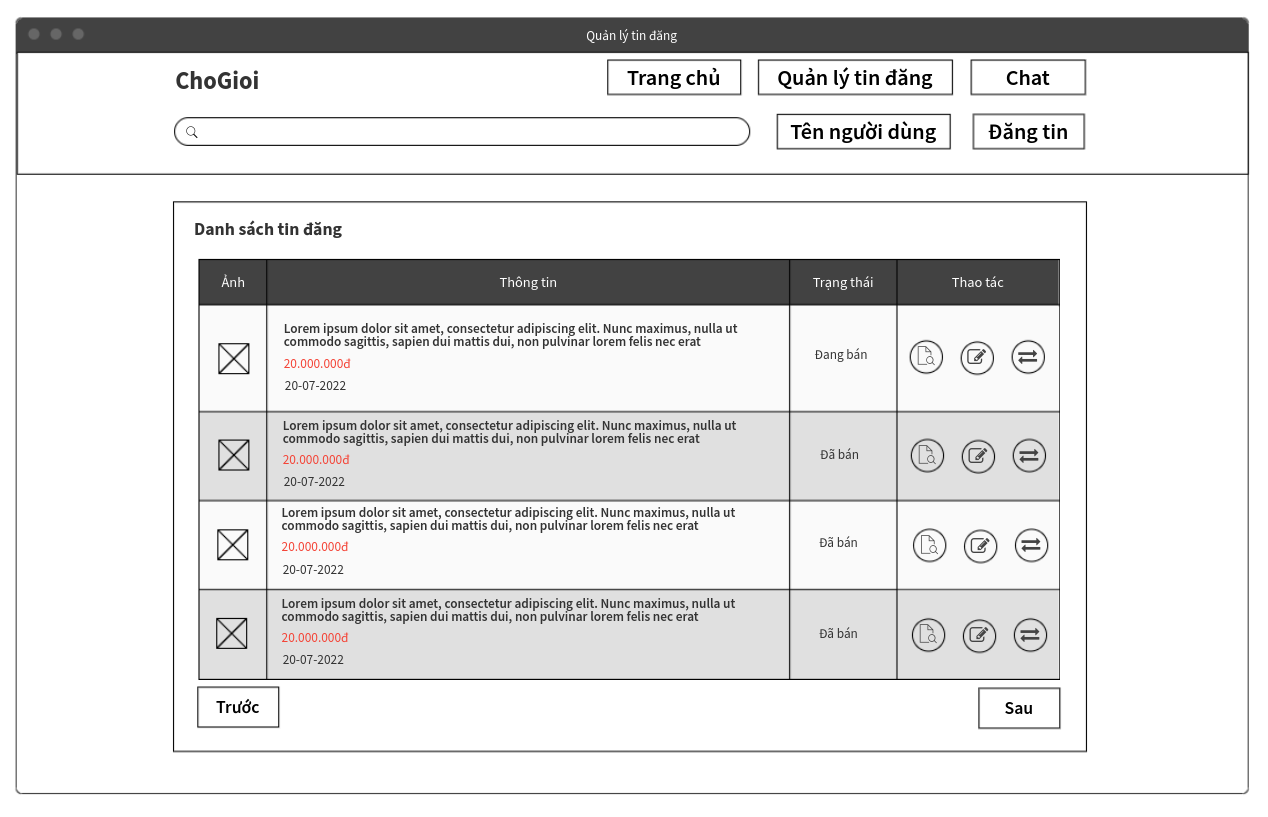
\includegraphics[width=0.8\linewidth]{Hinhve/PostManageMockup.png}
    \caption{Wireframe màn hình Quản lý bài đăng}
    \label{fig:Fig1}
\end{figure}
\newpage
\begin{figure}[H]
    \centering
    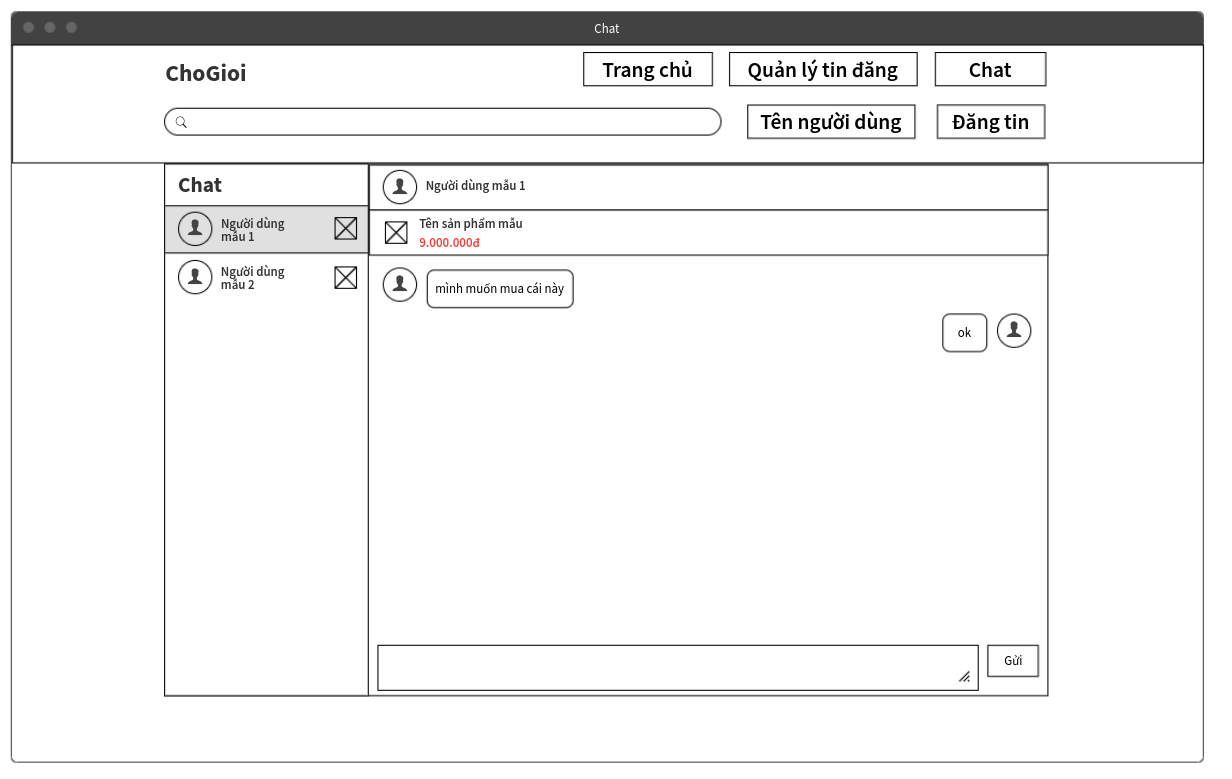
\includegraphics[width=0.8\linewidth]{Hinhve/chatMockup.png}
    \caption{Wireframe màn hình Chat}
    \label{fig:Fig1}
\end{figure}
\begin{figure}[H]
    \centering
    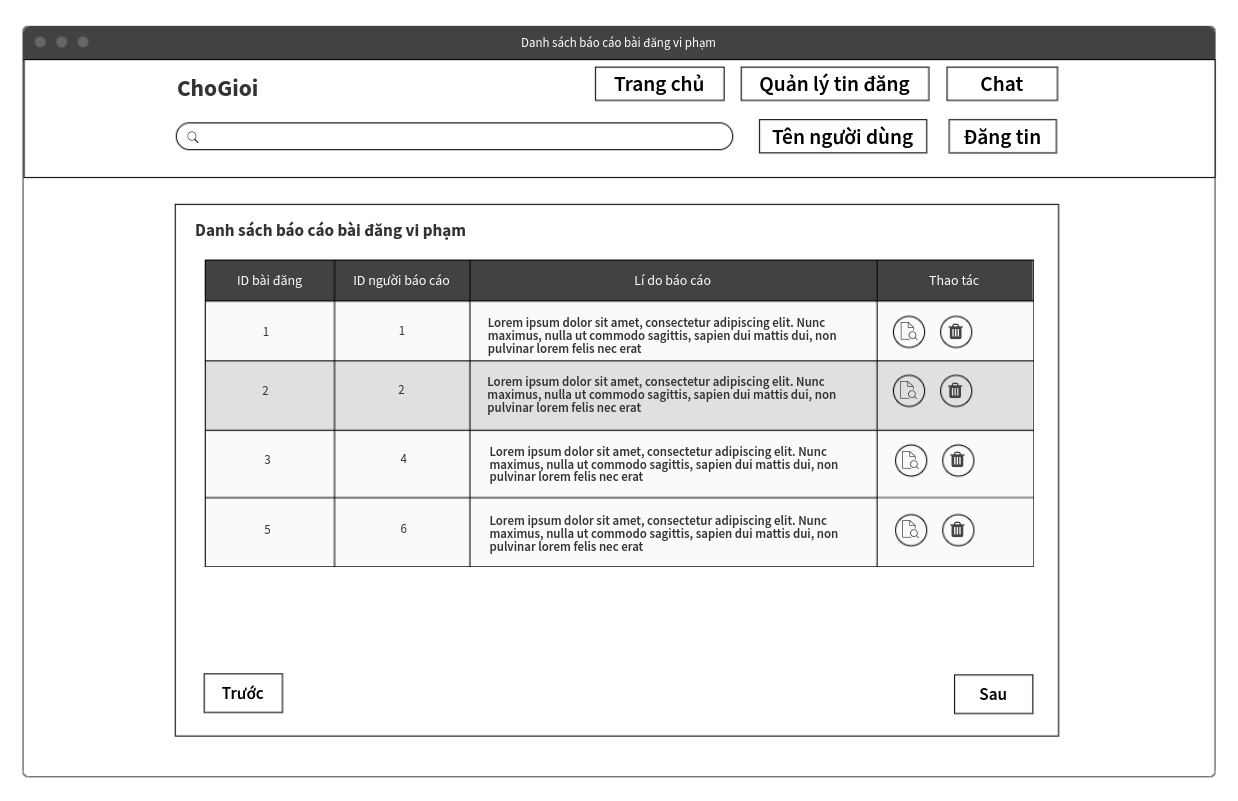
\includegraphics[width=0.8\linewidth]{Hinhve/reportMockup.png}
    \caption{Wireframe màn hình Quản lý Báo cáo}
    \label{fig:Fig1}
\end{figure}
\newpage
\subsection{Thiết kế lớp}
Phần này trình bày sơ đồ lớp chi tiết cho gói Database chứa các Model liên kết với các thực thể trong cơ sở dữ liệu. Sau đó sẽ là mô tả chi tiết cho một số lớp quan trọng nhất. Đồng thời, ĐATN sẽ minh họa việc thiết kế lớp bằng sơ đồ trình tự thể hiện luồng truyền thông điệp giữa các đối tượng của một số use case.

\begin{figure}[H]
    \centering
    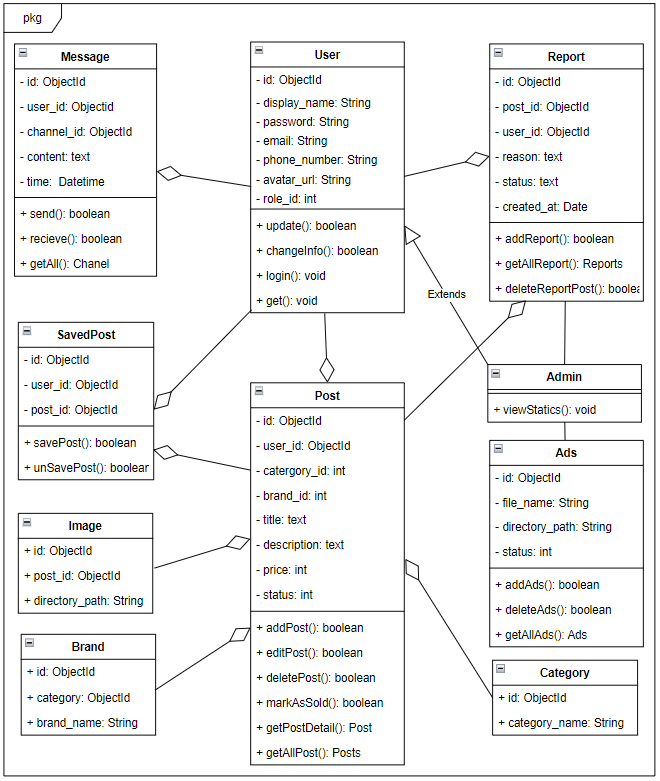
\includegraphics[width=0.95\linewidth]{Hinhve/thietkelop.png}
    \caption{Sơ đồ lớp chi tiết gói Database}
    \label{fig:Fig1}
\end{figure}
\newpage
\subsubsection{Mô tả lớp các lớp}
\begin{itemize}
    \item Lớp Post: Định nghĩa dữ liệu cho bảng Posts và quan hệ của nó với các bảng khác. Trong lớp Post có các phương thức sau:
        \begin{itemize}
            \item addPost() là phương thức Thêm bài đăng với đầu vào là thông tin dữ liệu và đầu ra ra là trạng thái boolean.
            \item editPost() là phương thức Cập nhật bài đăng với đầu vào là thông tin dữ liệu cập nhật và đầu ra là trạng thái boolean.
            \item deletePost() là phương thức Xóa bài đăng với đầu vào là id của bài đăng và đầu ra là trạng thái boolean.
            \item markAsSold() là phương thức Đánh dấu bài đăng đã được bán với đầu vào là id của bài đăng và đầu ra là trạng thái boolean.
            \item getPostDetail() là phương thức Lấy thông tin chi tiết của bài đăng với đầu vào là id của bài đăng và đầu ra là thông tin của bài đăng đó.
             \item getAllPost() là phương thức Lấy toàn bộ bài đăng. Phương thức này không có tham số đầu vào, đầu ra của phương thức là danh sách các bài đăng.
        \end{itemize}
    \item Lớp Message: Định nghĩa dữ liệu cho bảng Message và quan hệ của nó với các bảng khác. Trong lớp Message có các phương thức sau:
        \begin{itemize}
            \item send() là phương thức Gửi tin nhắn với đầu vào là thông tin user, bài đăng và nội dung tin nhắn, đầu ra là trạng thái boolean.
            \item receive() là phương thức  Nhận tin nhắn với đầu vào là thông tin user và bài đăng nhắn, đầu ra là trạng thái boolean.
            \item getAll() là phương thức Lấy ra tất cả danh sách cuộc trò chuyện của người dùng với đầu vào là thông tin user, đầu ra là các kênh chat.
        \end{itemize}
    \item Lớp Report: Định nghĩa dữ liệu cho bảng Report và quan hệ của nó với các bảng khác. Trong lớp Report có các phương thức sau:
        \begin{itemize}
            \item addReport() là phương thức Gửi báo cáo với đầu vào là thông tin user, bài đăng và lý do báo cáo, nhắn đầu ra là trạng thái boolean.
            \item getAllReport() là phương thức Lấy ra tất cả báo cáo. Phương thức này không có tham số đầu vào, đầu ra của phương thức là danh sách các báo cáo.
            \item deleteReportPost() là phương thức Xóa bài đăng bị báo cáo với đầu vào là id của bài đăng bị báo cáo và đầu ra là trạng thái boolean.
        \end{itemize}
    
\end{itemize}
\subsubsection{Sơ đồ trình tự cho một số use case}
\begin{figure}[H]
    \centering
    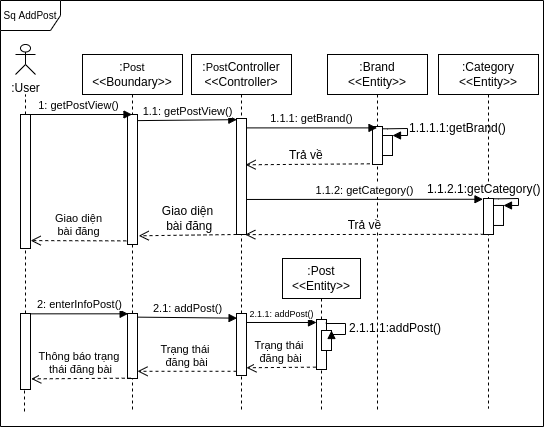
\includegraphics[width=0.85\linewidth]{Hinhve/PostSequence.png}
    \caption{Sơ đồ trình tự use case Thêm bài đăng}
    \label{fig:Fig1}
\end{figure}

\begin{figure}[H]
    \centering
    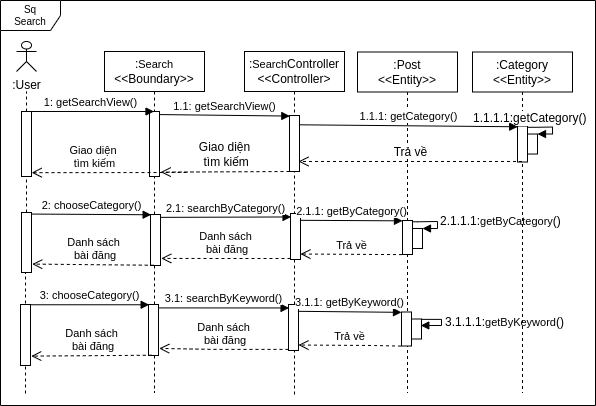
\includegraphics[width=0.85\linewidth]{Hinhve/SearchSequence.png}
    \caption{Sơ đồ trình tự use case Tìm kiếm bài đăng}
    \label{fig:Fig1}
\end{figure}
\newpage
\begin{figure}[H]
    \centering
    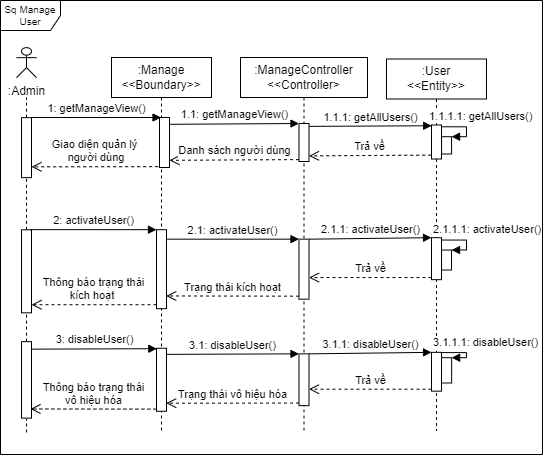
\includegraphics[width=0.85\linewidth]{Hinhve/ManageUserSequence.png}
    \caption{Sơ đồ trình tự use case Quản lý người dùng}
    \label{fig:Fig1}
\end{figure}
\begin{figure}[H]
    \centering
    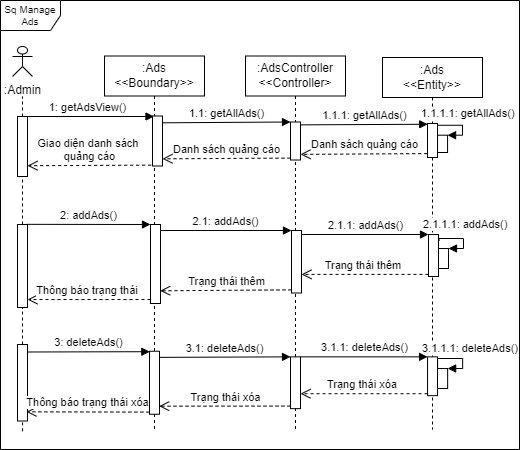
\includegraphics[width=0.85\linewidth]{Hinhve/adsSequence.png}
\caption{Sơ đồ trình tự use case Quản lý Quảng cáo}
    \label{fig:Fig1}
\end{figure}
\newpage
\subsection{Thiết kế API}
Mục này liệt kê danh sách các API được thiết kế và sử dụng trong hệ thống
\begin{table}[H]
\begin{tabular}{|p{1cm}|p{5.5cm}|p{1.5cm}|p{6.5cm}|}
\hline
STT & Mục đích                                             & Phương thức & Địa chỉ                           \\ \hline
1   & Đăng nhập                                            & POST        & api/user/login                    \\ \hline
2   & Đăng ký tài khoản                                    & POST        & api/user/register                 \\ \hline
3   & Đăng xuất                                            & POST        & api/user/logout                   \\ \hline
4   & Lấy thông tin cá nhân                                & GET         & api/user/me                       \\ \hline
5   & Tạo mới bài đăng                                     & POST        & api/user/create-post              \\ \hline
6   & Lấy ra thông tin chi tiết của một bài đăng           & GET         & api/user/posts                    \\ \hline
7   & Cập nhật bài đăng cá nhân                            & POST        & api/user/edit                     \\ \hline
8   & Lưu bài đăng của người khác                          & POST        & api/user/savePost                 \\ \hline
9   & Báo cáo bài viết                                     & POST        & api/user/reportPost               \\ \hline
10  & Xóa bài viết báo cáo                                 & POST        & api/user/deletePostOnReport       \\ \hline
11  & Lấy danh sách bài đăng của người dùng bất kì         & GET         & api/user/getAllPosts              \\ \hline
12  & Lấy danh sách bài đăng của người dùng đang đăng nhập & GET         & api/user/getAllPostsOfCurrentUser \\ \hline
13  & Lấy danh sách bài đăng đã lưu                        & GET         & api/user/getAllSavedPosts         \\ \hline
14  & Cập nhật thông tin cá nhân                           & POST        & api/user/updateUserInfo           \\ \hline
15  & Lấy danh sách nhãn hiệu                              & GET         & api/brands                        \\ \hline
16  & Thay đổi trạng thái của bài đăng                     & POST        & api/user/changePostStatus         \\ \hline
17  & Lấy thông tin người dùng bất kì                      & GET         & api/user/getUserById              \\ \hline
18  & Lấy danh sách quảng cáo                              & GET         & api/user/getAllAds                \\ \hline
19  & Tìm kiếm bài viết                                    & GET         & api/user/search                   \\ \hline
20  & Lấy danh sách tỉnh, thành phố                        & GET         & api/provinces                     \\ \hline
21  & Lấy danh sách quận, huyện theo tỉnh                  & GET         & api/districts                     \\ \hline
22  & Lấy danh sách phường, xã                             & GET         & api/wards                         \\ \hline
23  & Lấy địa chỉ đầy đủ                                   & GET         & api/fullAddressByWardId           \\ \hline
24  & Lấy thông tin Admin                                  & GET         & api/admin/me                      \\ \hline
25  & Đăng nhập Admin                                      & POST        & api/admin/login                   \\ \hline
26  & Đăng xuất Admin                                      & POST        & api/admin/logout                  \\ \hline
27  & Lấy danh sách bài viết bị báo cáo                    & GET         & api/admin/getAllReports           \\ \hline
28  & Xem thống kê bài đăng theo tháng                     & GET         & api/admin/postStatsByMonthInYear  \\ \hline
29  & Xem thống kê người dùng theo năm                     & GET         & api/admin/userStatsByMonthInYear  \\ \hline
\end{tabular}
\caption{Danh sách API được sử dụng trong hệ thống phần 1}
\label{tab:my-table}
\end{table}
\newpage
\begin{table}[H]
\begin{tabular}{|p{1cm}|p{5.5cm}|p{1.5cm}|p{6.5cm}|}
\hline
STT & Mục đích                                       & Phương thức & Địa chỉ                       \\ \hline
30  & Xem thống kê bài đăng theo danh mục            & GET         & api/admin/postStatsByCategory \\ \hline
31  & Lấy số lượng bài đăng trong hệ thống           & GET         & api/admin/allPostsCount       \\ \hline
32  & Lấy số lượng sản phẩm đã được mua bán          & GET         & api/admin/soldPostsCount      \\ \hline
33  & Lấy số lượng người dùng trong hệ thống         & GET         & api/admin/allUsersCount       \\ \hline
34  & Lấy danh sách người dùng                       & GET         & api/admin/getAllUsers         \\ \hline
35  & Thiết lập trạng thái người dùng                & POST        & api/admin/toggleBlockUser     \\ \hline
36  & Cập nhật thông tin người dùng bằng quyền Admin & POST        & api/admin/updateUserInfo      \\ \hline
37  & Lấy danh sách quảng cáo cho quyền Admin        & GET         & api/admin/getAllAds           \\ \hline
38  & Thêm quảng cáo                                 & POST        & api/admin/addAds              \\ \hline
39  & Thay đổi trạng thái quảng cáo                  & POST        & api/admin/toggleStatusAds     \\ \hline
\end{tabular}
\caption{Danh sách API được sử dụng trong hệ thống phần 2}
\label{tab:my-table}
\end{table}
\newpage
\subsection{Thiết kế cơ sở dữ liệu}
Mục này trình bày về việc thiết kế cơ sở dữ liệu bằng cách minh họa sơ đồ thực thể liên kết và mô tả các thực thể tương ứng trong cơ sở dữ liệu của hệ thống.
\subsubsection{Tổng quan cơ sở dữ liệu}
\begin{figure}[H]
    \centering
    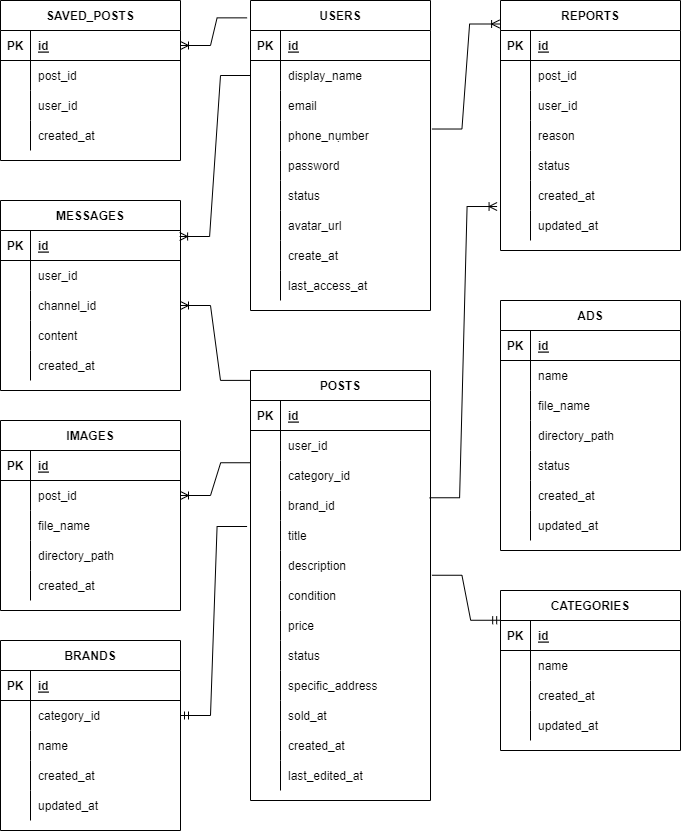
\includegraphics[width=0.95\linewidth]{Hinhve/entity.png}
    \caption{Sơ đồ thực thể liên kết}
    \label{fig:Fig1}
\end{figure}
\newpage
Các bảng dữ liệu chính tham gia trực tiếp vào các ca sử dụng chính của hệ thống: 
\begin{itemize}
    \item USERS (id, display$\_$name, email, phone$\_$number, password, status, avatar$\_$url, created$\_$at, last$\_$acess$\_$at)
    \item POSTS (id, user$\_$id, category$\_$id, brand$\_$id, title, description, condition, price, status, specific$\_$address, sold$\_$at, created$\_$at, last$\_$edited$\_$at) 
    \item IMAGES (id, post$\_$id, file$\_$name, directory$\_$path, created)
    \item SAVED$\_$POSTS (id, post$\_$id, user$\_$id, created$\_$at)
    \item REPORTS (id, post$\_$id, user$\_$id, reason, status, created$\_$at, updated$\_$at)  
    \item CATEGORIES (id, name, created$\_$at, update$\_$at) 
    \item BRANDS (id, category$\_$id, name, created$\_$at, update$\_$at)
    \item MESSAGES (id, user$\_$id, channel$\_$id, content, created$\_$at)
    \item ADS (id, name, file$\_$name, directory$\_$path, status, created$\_$at, update$\_$at)
\end{itemize}

Phần sau đây sẽ mô tả chi tiết từng bảng được thiết kế và sử dụng trong hệ thống. Các thông tin được mô tả bao gồm: Tên trường, Kiểu dữ liệu, Required/Not Required (Bắt buộc hay không bắt buộc), Ghi chú.
\subsubsection{Mô tả chi tiết các bảng trong cơ sở dữ liệu}
\begin{table}[H]
\centering
\begin{tabular}{|p{2.7cm}|l|p{2.5cm}|p{4cm}|}
\hline
Tên trường       & Kiểu     & Required/   Not Required & Ghi chú                       \\ \hline
id               & ObjectId & Required                 & UserId                        \\ \hline
display\_name    & String   & Required                 & Tên hiển thị                  \\ \hline
email            & String   & Required                 & Email cá nhân                 \\ \hline
phone\_number    & String   & Required                 & Số điện thoại                 \\ \hline
password         & String   & Required                 & Mật khẩu                      \\ \hline
avatar\_url      & String   & Not Required             & Đường dẫn ảnh   đại diện      \\ \hline
created\_at      & Datetime & Required                 & Thời gian tạo                 \\ \hline
update\_at       & Datetime & Not Required             & Thời gian cập   nhật          \\ \hline
last\_access\_at & Datetime & Not Required             & Thời gian truy   cập mới nhất \\ \hline
\end{tabular}
\caption{Mô tả chi tiết bảng Users}
\label{tab:my-table}
\end{table}
\newpage
\begin{table}[H]
\centering
\begin{tabular}{|p{2.9cm}|l|p{2.5cm}|p{4cm}|}
\hline
Tên trường        & Kiểu     & Required/ Not Required & Ghi chú                                                              \\ \hline
id                & ObjectId & Required               & PostId                                                               \\ \hline
user\_id          & ObjectId & Required               & \begin{tabular}[c]{@{}l@{}}UserId\\ Ref: Users\end{tabular}          \\ \hline
category\_id      & ObjectId & Required               & \begin{tabular}[c]{@{}l@{}}CategoryId\\ Ref: Categories\end{tabular} \\ \hline
title             & Text     & Required               & Tiêu đề                                                              \\ \hline
description       & Text     & Required               & Mô tả                                                                \\ \hline
condition         & String   & Required               & Tình trạng                                                           \\ \hline
price             & Int      & Required               & Giá                                                                  \\ \hline
status            & String   & Required               & Trạng thái                                                           \\ \hline
specific\_address & String   & Required               & Địa chỉ cụ thể                                                       \\ \hline
sold\_at          & Datetime & Required               & Thời gian bán                                                        \\ \hline
created\_at       & Datetime & Required               & Thời gian tạo                                                        \\ \hline
update\_at        & Datetime & Not Required           & Thời gian cập   nhật                                                 \\ \hline
\end{tabular}
\caption{Mô tả chi tiết bảng Posts}
\label{tab:my-table}
\end{table}
\begin{table}[H]
\centering
\begin{tabular}{|p{2.5cm}|l|p{2.5cm}|p{4cm}|}
\hline
Tên trường  & Kiểu     & Required/ Not Required & Ghi chú                                                            \\ \hline
id          & ObjectId & Required               & RoleId                                                             \\ \hline
post\_id    & ObjectId & Required               & \begin{tabular}[c]{@{}l@{}}Mã bài viết\\ Ref: POSTS\end{tabular}   \\ \hline
user\_id    & ObjectId & Required               & \begin{tabular}[c]{@{}l@{}}Mã người dùng\\ Ref: USERS\end{tabular} \\ \hline
created\_at & Datetime & Required               & Thời gian tạo                                                      \\ \hline
update\_at  & Datetime & Not Required           & Thời gian cập   nhật                                               \\ \hline
\end{tabular}
\caption{Mô tả chi tiết bảng Saved$\_$posts}
\label{tab:my-table}
\end{table}
\begin{table}[H]
\centering
\begin{tabular}{|p{2.5cm}|l|p{2.5cm}|p{4cm}|}
\hline
Tên trường  & Kiểu     & \begin{tabular}[c]{@{}l@{}}Required/ Not\\  Required\end{tabular} & Ghi chú                                                             \\ \hline
id          & ObjectId & Required                                                               & ReportId                                                            \\ \hline
post\_id    & ObjectId & Required                                                               & \begin{tabular}[c]{@{}l@{}}Mã bài viết\\ Ref: POSTS\end{tabular}    \\ \hline
user\_id    & ObjectId & Required                                                               & \begin{tabular}[c]{@{}l@{}}Mã người dùng \\ Ref: USERS\end{tabular} \\ \hline
reason      & String   & Required                                                               & Lý do báo cáo                                                       \\ \hline
status      & String   & Required                                                               & Trạng thái xử lý                                                    \\ \hline
created\_at & Datetime & Required                                                               & Thời gian tạo                                                       \\ \hline
update\_at  & Datetime & Not Required                                                           & Thời gian cập   nhật                                                \\ \hline
\end{tabular}
\caption{Mô tả chi tiết bảng Reports}
\label{tab:my-table}
\end{table}
\begin{table}[H]
\centering
\begin{tabular}{|p{2.5cm}|l|p{2.5cm}|p{4cm}|}
\hline
Tên trường      & Kiểu     & Required/ Not Required & Ghi chú                \\ \hline
id              & ObjectId & Required               & ImageId                \\ \hline
name            & String   & Required               & Tên quảng cáo          \\ \hline
file\_name      & String   & Required               & Tên file               \\ \hline
directory\_path & String   & Required               & Đường   dẫn đến ảnh    \\ \hline
status          & String   & Required               & Trạng   thái quảng cáo \\ \hline
created\_at     & Datetime & Required               & Thời gian tạo          \\ \hline
update\_at      & Datetime & Not Required           & Thời gian cập   nhật   \\ \hline
\end{tabular}
\caption{Mô tả chi tiết bảng Ads}
\label{tab:my-table}
\end{table}
\begin{table}[H]
\centering
\begin{tabular}{|p{2.5cm}|l|p{2.5cm}|p{4cm}|}
\hline
Tên trường      & Kiểu     & Required/ Not Required & Ghi chú                                                           \\ \hline
id              & ObjectId & Required               & ImageId                                                           \\ \hline
postId          & ObjectId & Required               & \begin{tabular}[c]{@{}l@{}}Mã bài viết\\  Ref: POSTS\end{tabular} \\ \hline
file\_name      & String   & Required               & Tên file                                                          \\ \hline
directory\_path & String   & Required               & Đường   dẫn đến ảnh                                               \\ \hline
created\_at     & Datetime & Required               & Thời gian tạo                                                     \\ \hline
update\_at      & Datetime & Not Required           & Thời gian cập   nhật                                              \\ \hline
\end{tabular}
\caption{Mô tả chi tiết bảng Images}
\label{tab:my-table}
\end{table}\newpage
\section{Xây dựng ứng dụng}
\subsection{Thư viện và công cụ sử dụng}
Mục này liệt kê danh sách các công cụ và thư viện đã sử dụng trong quá trình thực hiện và xây dựng đồ án. Những công cụ này đã hỗ trợ ĐATN xuyên suốt quá trình từ phân tích thiết kế cho tới bước lập trình.
\begin{table}[H]
\centering
\begin{tabular}{|p{3.5cm}|p{3.6cm}|p{5.5cm}|}
\hline
Mục đích                            & Công cụ            & Địa chỉ URL                    \\ \hline
IDE lập trình                       & Visual Studio Code & https://code.visualstudio.com/ \\ \hline
Ngôn ngữ lập trình Frontend         & Javascript         & https://www.javascript.com/    \\ \hline
\multirow{2}{*}{Thư viện giao diện} & ReactJS 16.13.1      & https://reactjs.org/           \\ \cline{2-3} 
                                    & Chakra UI 1.4.11   & https://chakra-ui.com/         \\ \hline
Ngôn ngữ lập trình Backend          & PHP 7.3            & https://www.php.net/           \\ \hline
Framework                           & Laravel 8          & https://laravel.com/           \\ \hline
\multirow{2}{*}{Quản trị CSDL}      & MySQL              & https://www.mysql.com/         \\ \cline{2-3} 
                                    & Firebase           & https://firebase.google.com/   \\ \hline
\multirow{2}{*}{Thiết kế}      & Diagrams.net             & https://www.diagrams.net/          \\ \cline{2-3} 
& MockFlow           & https://www.mockflow.com/   \\ \hline
\end{tabular}
\caption{Danh sách công cụ và thư viện sử dụng}
\label{tab:my-table}
\end{table}
\newpage
\subsection{Minh họa các chức năng chính}
Trong phần này, ĐATN sẽ lựa chọn và đưa ra minh họa các màn hình của những chức năng chính của hệ thống.
\subsubsection{Màn hình trang chủ phía người dùng}
\begin{figure}[H]
    \centering
    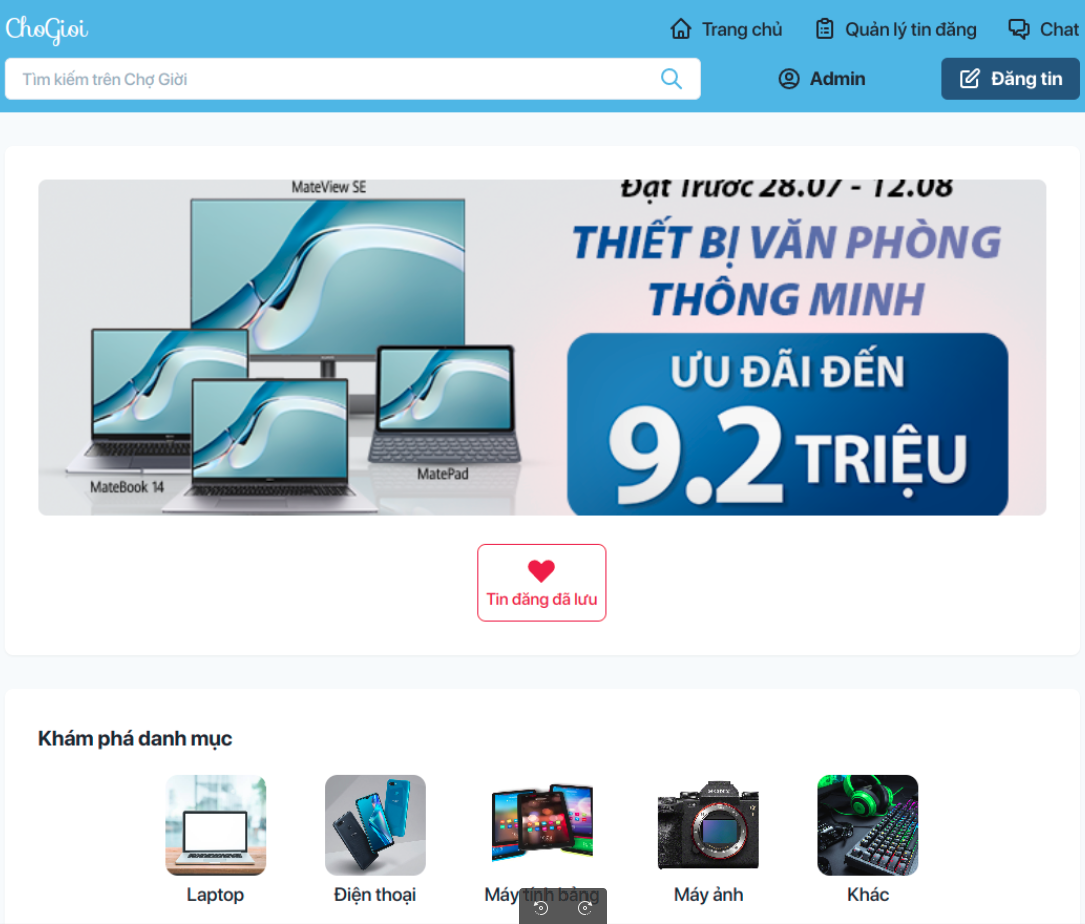
\includegraphics[width=0.9\linewidth]{Hinhve/1-home.png}
    \caption{Màn hình trang chủ phía người dùng}
    \label{fig:Fig1}
\end{figure}
Hình 4.14 phía trên là màn hình trang chủ của người dùng sau khi đăng nhập vào hệ thống. Phía trên cùng là thanh chứa hầu hết các chức năng của hệ thống. Đầu tiên, phía bên trái là thanh tìm kiếm giúp người dùng có thể tìm kiếm hệ thống theo từ khóa. Phía bên phải của thanh này người còn có thể sử dụng các chức năng như Quản lý tin đăng, Đăng tin, Vào danh sách Chat và Quản lý thông tin cá nhân. Phía trung tâm của màn hình là phần hiển thị của các quảng cáo từ nhà tài trợ. Phía dưới banner quảng cáo người dùng có thể lựa chọn chức năng xem danh sách tin đăng đã lưu. Phía dưới cùng của màn hình là các danh mục chính của hệ thống, khi click vào 1 danh mục bất kì hệ thống sẽ hiển thị ra danh sách các bài đăng tương ứng với danh mục đó
\newpage
\subsubsection{Màn hình Tìm kiểm sản phẩm}
\begin{figure}[H]
    \centering
    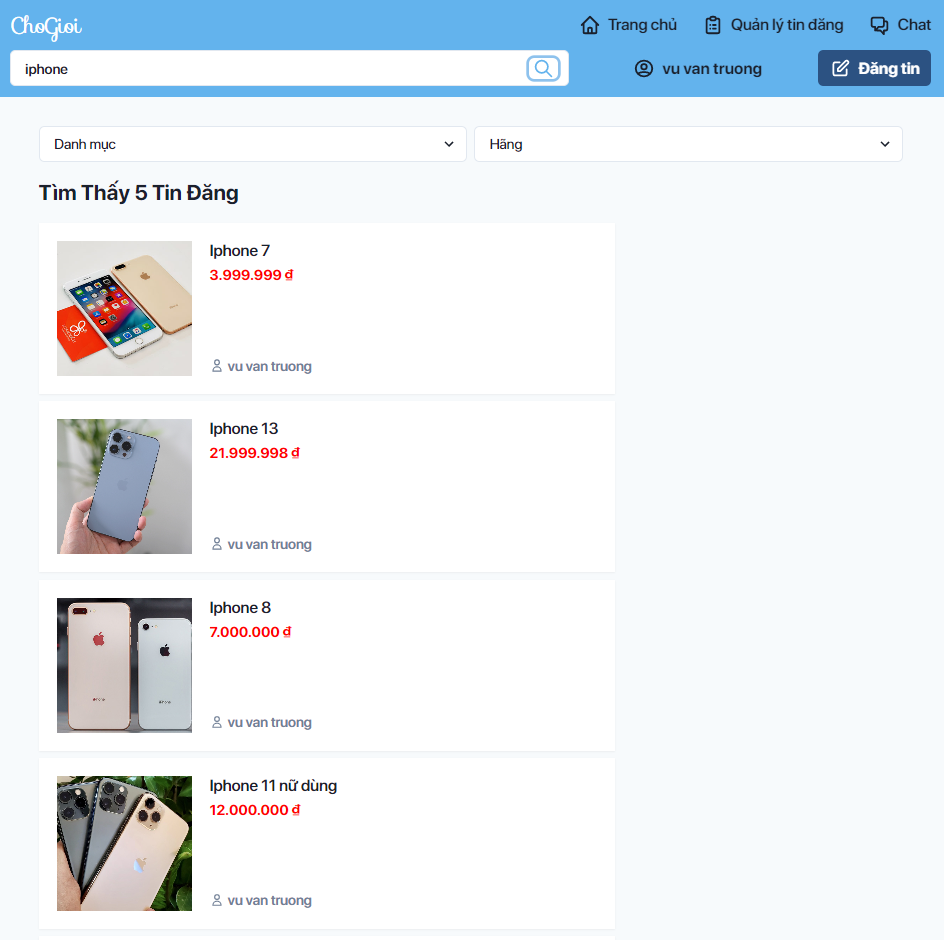
\includegraphics[width=0.9\linewidth]{Hinhve/2-search.png}
    \caption{Màn hình Tìm kiếm sản phẩm}
    \label{fig:Fig1}
\end{figure}
Đây là màn hình tìm kiếm sản phẩm của thệ thống. Người dùng có thể nhập từ khóa tìm kiếm vào thanh tìm kiếm phía trên  cùng của màn hình. Ở màn hình trang chủ, sau khi người dùng nhập từ khóa tìm kiếm và nhấn tìm kiếm từ hệ thống sẽ điều hướng đến trang Tìm kiếm. Có thể thấy sau khi nhập từ khóa "iphone" hệ thống sẽ hiển thị ra danh sách các sản phẩm liên quan tương ứng. Đặc biệt ở màn hình này, chỉ cần nhập từ 3 ký tự trở lên, hệ thống sẽ tự động hiển thị những sản phẩm có nội dung liên quan mà không cần người dùng phải click vào nút tìm kiếm. Ngoài ra, ở màn hình này người dùng còn có thể lọc bài đăng theo danh mục hoặc hãng sản xuất.
\newpage
\subsubsection{Màn hình Quản lý tin đăng}
\begin{figure}[H]
    \centering
    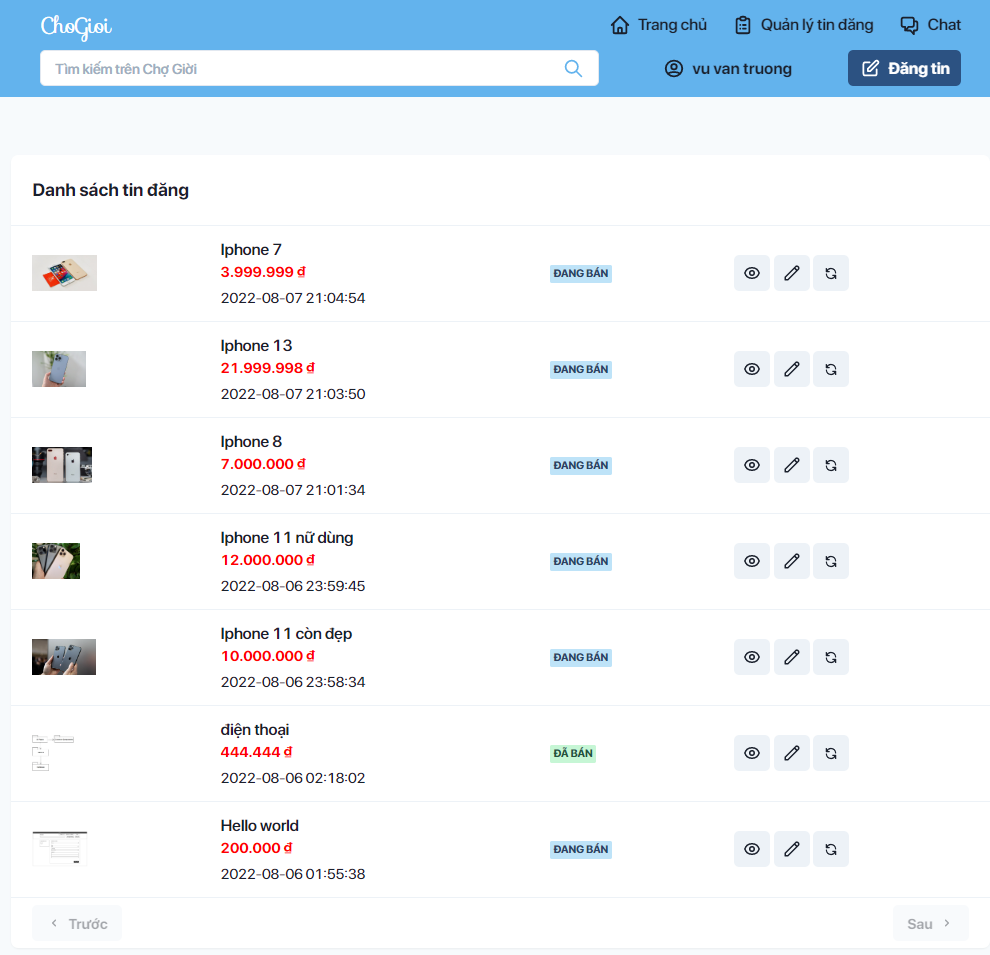
\includegraphics[width=0.9\linewidth]{Hinhve/3-manage.png}
    \caption{Màn hình Quản lý tin đăng}
    \label{fig:Fig1}
\end{figure}
Ở màn hình Quản lý tin đăng, danh sách các bài đăng của người dùng được hiển thị với các trạng thái là Đang bán hoặc Đã bán. Phía bên phải của mỗi bài đăng là 3 nút tương ứng với các chức năng Xem chi tiết bài đăng, Cập nhật bài đăng và Thiết lập trạng thái bài đăng.
\newpage
\subsubsection{Màn hình Chat}
\begin{figure}[H]
    \centering
    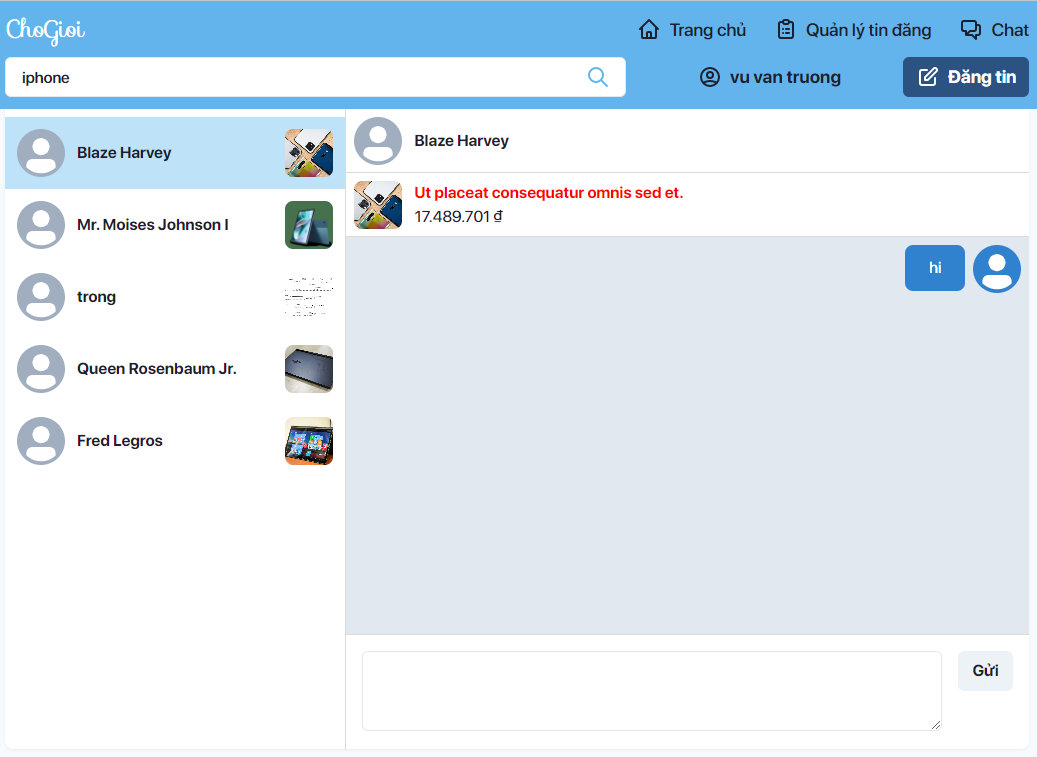
\includegraphics[width=0.9\linewidth]{Hinhve/4-chat.png}
    \caption{Màn hình Chat}
    \label{fig:Fig1}
\end{figure}
Trong màn hình này, danh sách các cuộc nói chuyện được liệt kê phía bên trái màn hình. Khi người dùng chọn cuộc trò chuyện tương ứng, nội dung cuộc trò chuyện sẽ được hiển thị phía bên phải màn hình. Trong cuộc hội thoại, ngoài tin nhắn trao đổi mua bán ra, hệ thống liên kế đến bài đăng ban đầu và hiển thị nó ở phía trên cuộc trò chuyện giúp người dùng có thể xem lại bài đăng bất cứ lúc nào.
\newpage
\subsubsection{Màn hình Admin}
\begin{figure}[H]
    \centering
    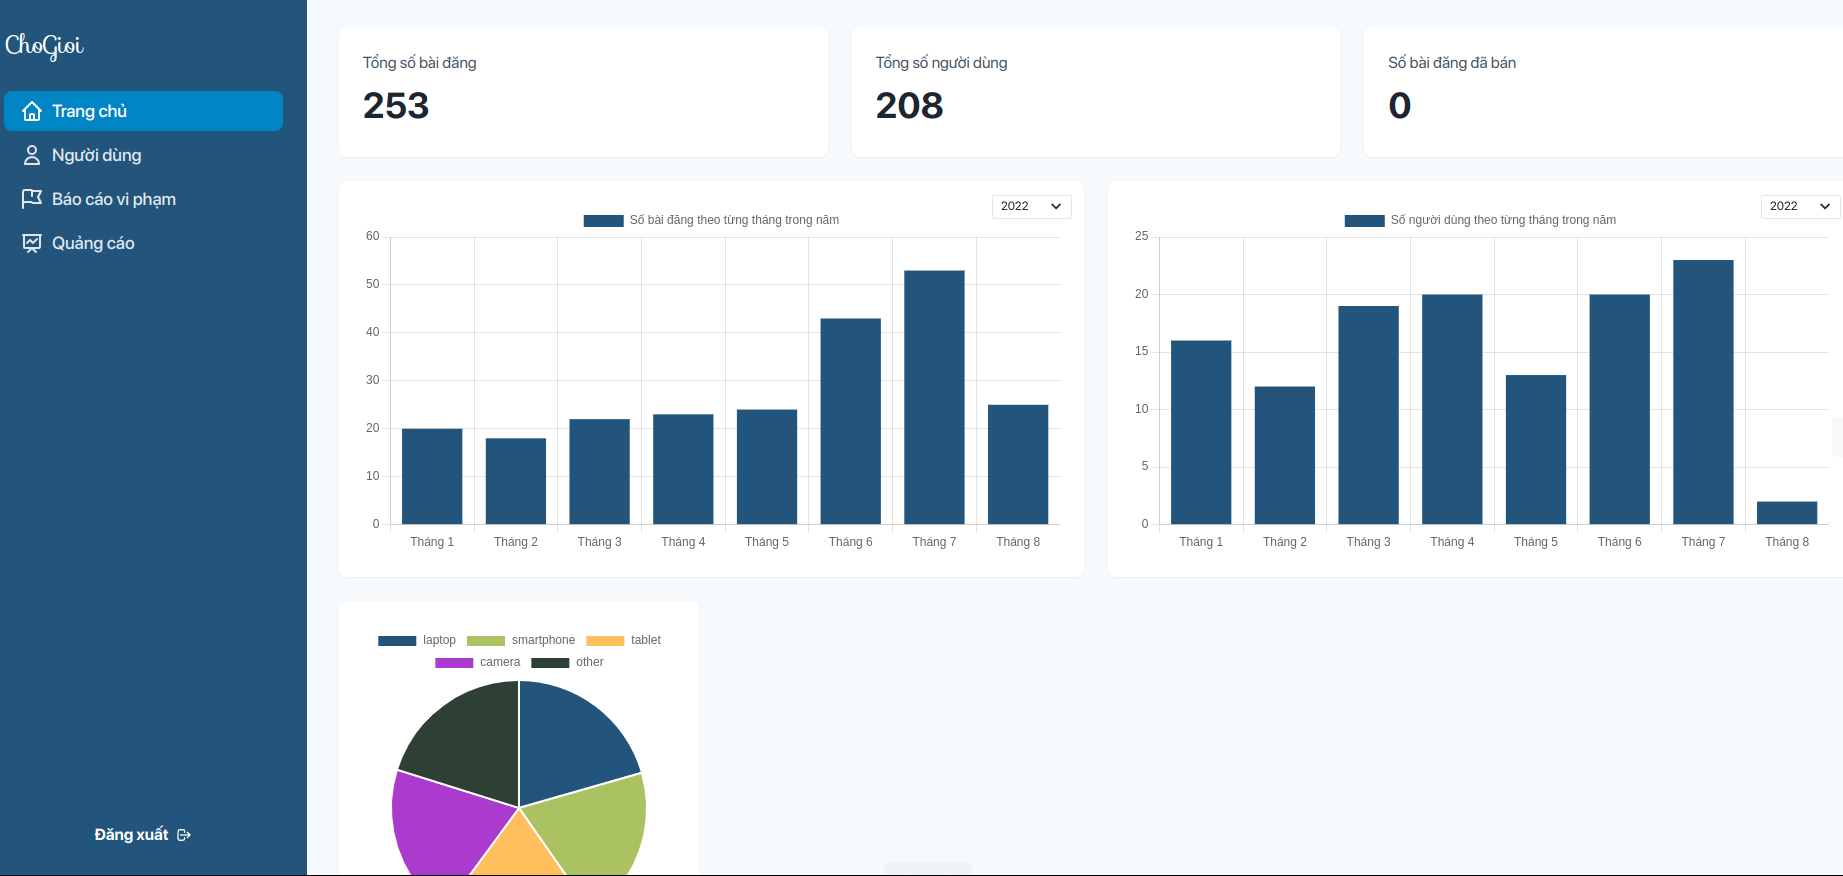
\includegraphics[width=0.99\linewidth]{Hinhve/6-admin.png}
    \caption{Màn hình Trang chủ Admin}
    \label{fig:Fig1}
\end{figure}
Khi Admin đăng nhập vào hệ thống, giao diện trang chủ của Admin sẽ được hiển thị. Nội dung được hiển thị ngay lập tức là những thống kê chung của hệ thống. Admin có thể xem được tổng số bài đăng, tổng số người dùng và tổng số bài đăng đã bán ở phía trên cùng của màn hình. Ở phần trung tâm của màn hình là các biểu đồ minh họa trực quan các thống kê theo thời gian, danh mục. Admin có thể lọc biểu đồ theo từng năm bằng cách thay đổi lựa chọn năm ở phía trên các biểu đồ cột. Ngoài ở màn màn hình trang chủ, ở side-bar admin có thể lựa chọn các chức năng khác của hệ thống bao gồm: Quản lý người dùng, Quản lý báo cáo vi phạm, Quản lý Quảng cáo.
\newpage
\section{Kiểm thử}
Sau khi thiết kế và xây dựng hệ thống, ĐATN thực hiện kĩ thuật Black-box để thực hiện kiểm thử các chức năng của hệ thống. Môi trường kiểm thử là các trình duyệt phổ biến tại Việt Nam như Chrome, Cốc Cốc và Firefox. Chi tiết các trường hợp kiểm thử của một số chức năng được mô tả phía dưới.
\subsection{Kiểm thử cho chức năng Đăng bài}
\begin{table}[H]
\begin{tabular}{|p{1cm}|p{5cm}|p{6cm}|p{1.5cm}|}
\hline
STT & Hành động                                                                 & Mong muốn                                                                         & Kết quả \\ \hline
1   & Không nhập thông tin một hoặc các trường bắt buộc nhưng vẫn nhấn Đăng bài & Hiển thị text màu đỏ yêu cầu nhập trường tương ứng phía dưới các trường chưa nhập & Đạt     \\ \hline
2   & Nhập tiêu đề quá 50 ký tự hoặc mô tả quá 1500 ký tự                       & Hiển thị text màu đỏ thông báo đã nhập quá số ký tự cho phép                      & Đạt     \\ \hline
3   & Nhập chữ vào trường "Giá"                                                 & Không cho phép, chỉ cho phép nhập số                                              & Đạt     \\ \hline
4   & Click vào ô chọn hãng                                                     & Lấy ra đầy đủ các hãng có trong hệ thống và lựa chọn được                         & Đạt     \\ \hline
5   & Click vào ô chọn danh mục                                                     & Lấy ra đầy đủ các danh mục có trong hệ thống và lựa chọn được                         & Đạt     \\ \hline
6   & Nhập đầy đủ thông tin hợp lệ và nhấn Đăng bài                             & Thông báo đăng bài thành công và lưu trữ thành công vào hệ thống                  & Đạt     \\ \hline
\end{tabular}
\caption{Kiểm thử cho chức năng Đăng bài}
\subsection{Kiểm thử cho chức năng Quản lý bài đăng}
\begin{table}[H]
\begin{tabular}{|p{1cm}|p{5cm}|p{6cm}|p{1.5cm}|}
\hline
STT & Hành động                                                & Mong muốn                                                                 & Kết quả \\ \hline
1   & Chọn biểu tượng biểu tượng hình con mắt của một bài viết & Mở ra một tab mới chứa thông tin bài đăng vừa chọn                        & Đạt     \\ \hline
2   & Chọn biểu tượng thay đổi trạng thái Đã bán/ Chưa bán     & Hiển thị pop-up cho phép thay đổi trạng thái và cập nhật tại màn hình này & Đạt     \\ \hline
3   & Chọn biểu tượng chỉnh sửa bài đăng                       & Hiển thị trang cập nhật và hiển thị đúng thông tin cũ của bài đăng đó     & Đạt     \\ \hline
4   & Nhập đầy đủ thông tin hợp lệ và chọn Cập nhật            & Thông báo trạng thái thành công và cập nhật thông tin vào hệ thống        & Đạt     \\ \hline
5   & Nhập thiếu các trường thông tin khi cập nhật bài đăng    & Hiển thị text màu đỏ yêu cập nhập trường thông tin bị thiếu               & Đạt     \\ \hline
\end{tabular}
\caption{Kiểm thử cho chức năng Quản lý bài đăng}
\label{tab:my-table}
\end{table}
\label{tab:my-table}
\end{table}

\begin{table}[H]
\centering
\begin{tabular}{|p{1cm}|p{5cm}|p{6cm}|p{1.5cm}|}
\hline
STT & Hành động                                                   & Mong muốn                                                                                 & Kết quả \\ \hline
1   & Chọn biểu tượng chat trong trang bài đăng                   & Hiển thị ra giao diện chat với người dùng và bài đăng ở trang trước                       & Đạt     \\ \hline
2   & Soạn tin nhắn và nhấn gửi                                   & Gửi thành công và người nhận nhận được tin nhắn                                           & Đạt     \\ \hline
3   & Chọn chức năng Chat ở màn hình trang chủ                    & Hiển thị danh sách các cuộc trò chuyện mua hoặc bán sản phẩm                              & Đạt     \\ \hline
4   & Chọn một người dùng trong danh sách cuộc trò chuyện         & Lấy được thông tin cuộc trò chuyện và lịch sử các tin nhắn từ trước                       & Đạt     \\ \hline
5   & Chọn thanh bài đăng được gắn phía trong mỗi cuộc trò chuyện & Mở ra một tab mới chứa thông tin bài đăng tương ứng với cuộc trò chuyện lựa chọn trước đó & Đạt     \\ \hline
\end{tabular}
\caption{Kiểm thử cho chức năng Quản lý Chat}
\label{tab:my-table}
\end{table}
\section{Triển khai}
\begin{table}[H]
\centering
\begin{tabular}{|l|l|}
\hline
Loại công cụ/thiết bị & Yêu cầu                         \\ \hline
Hệ điều hành                   & Hệ điều hành Windows phiên bản 7 trở lên \\ \hline
CPU                            & Bộ xử lý 2 nhân, tối thiểu 1.8 GHz       \\ \hline
GPU                            & Không yêu cầu                            \\ \hline
Ram                            & Tối thiểu 2GB                            \\ \hline
Bộ nhớ                         & Trống tối thiểu 4GB                      \\ \hline
\end{tabular}
\caption{Danh sách công cụ/thiết bị triển khai hệ thống}
\label{tab:my-table}
\end{table}
Hệ thống được triển khai trên localhost. Trình tự thực hiện được liệt kê lần lượt theo các bước sau đây:
\begin{itemize}
    \item Bước 1: Cài đặt Composer bản mới nhất.
    \item Bước 2: Cài đặt PHP version 7.3.
    \item Bước 3: Cài đặt Node version 16 stable
    \item Bước 4: Cài đặt hệ quản trị cơ sở dữ liệu MySQL.
    \item Bước 5: Tạo file biến môi trường từ file mẫu bằng lệnh: "cp .env.example .env".
    \item Bước 6: Tạo cơ sở dữ liệu bằng MySQL rồi cập nhật trong file .env các trường sau: DB$\_$DATABASE, DB$\_$USERNAME, DB$\_$PASSWORD.
    \item Bước 7: Cài đặt các gói thư viện PHP: "composer install"
    \item Bước 8: Tạo app key: "php artisan key:generate".
    \item Bước 9: Tạo JWT key (cho việc xác thực): "php artisan jwt:secret".
    \item Bước 10: Chạy lệnh migration để tạo các bảng, đồng thời tạo dữ liệu ảo: "php artisan migrate --seed".
    \item Bước 11: Cài các gói thư viện Javascript:
"npm install".
    \item Bước 12:  Thực hiện Build giao diện:
"npm run prod".
    \item Bước 13:  Khởi chạy server: "php artisan serve".



\end{itemize}
\end{document}
